\def\baselinestretch{1}
\chapter{Agrupamiento de series temporales}
\def\baselinestretch{1.0}
\goodbreak
%%%------------Introduccion---------------------------------------
\section{Introducci\'on}
En este Cap\'itulo se dar\'a una definici\'on del \'Indice de Disimilaridad, para as\'i implementar una medida con el cual se trabajar\'a para la
clasificaci\'on de series temporales.

La motivaci\'on de analizar el comportamiento de un par de series temporales, es mayor a\'un cuando \'este se extiende para un conjunto de series temporales.

Ahora bien, como s\'imil al an\'alisis de cluster, es necesario extender algunos m\'etodos ya conocidos de agrupaci\'on, para un conjunto de variables aleatorias a trav\'es del tiempo. La variaci\'on de esta t\'ecnica, es considerar la informaci\'on del comovimiento a trav\'es del tiempo de los distintos pares de series temporales, donde el an\'alisis multivariante cl\'asico no considera.

El an\'alisis por agrupaci\'on (Cluster analysis) es una t\'ecnica
muy utilizada en problemas multivariados donde se quiere agrupar
unidades experimentales con ciertas caracter\'isticas o
generalizar grupo de variables de inter\'es. El objetivo
de este Cap\'itulo es definir algunas t\'ecnicas de
agrupaci\'on. Las t\'ecnicas m\'as usadas en este contexto son:

\begin{enumerate}
  \item M\'etodos de agrupaci\'on no jer\'arquicos.
  \item M\'etodos de agrupaci\'on jer\'arquicos.
\end{enumerate}
Estas definiciones ayudar\'an de base para definir una nueva medida de proximidad entre series temporales, asociados a las t\'ecnicas cl\'asicas de agrupaci\'on.
\section{M\'etodos de Agrupaci\'on}
Dependiendo del m\'etodo de agrupaci\'on que utilicemos los resultados finales variar\'an. Entonces, cada m\'etodo tiene una caracter\'istica en particular que es necesario considerar, en esta secci\'on se estudiar\'an los siguientes m\'etodos de agrupaci\'on:
\begin{enumerate}
  \item \textbf{M\'etodos de agrupaci\'on no jer\'arquicos}
   Se usan para agrupar objetos en un conjunto de k-cluster
  predeterminados, se parte de un conjunto inicial de clusters
  elegidos al azar luego se van cambiando de modo iterativo, habitualmente se usa el m\'etodo de las k-medias.
  \\\textbf{M\'etodo de las k-medias}
  \\Es un m\'etodo que permite asignar a cada observaci\'on el cluster
  que se encuentra m\'as pr\'oximo en t\'erminos el centroide (Valor medio de las observaciones de las variables en el valor del
  conglomerado).
  \begin{itemize}
  \item Se eligen al azar k-clusters iniciales.
  \item Para el conjunto de observaciones se vuelve a calcular la
  distancia al centroide de los clusters y se reasignan a los que
  est\'an mas pr\'oximos. Se vuelven a calcular los centroides de los
  k-cluster despu\'es de las reasignaciones de los elementos.
  \item Se repiten los pasos anteriores hasta que no se produzca
  ninguna reasignaci\'on.
  \end{itemize}
  \item \textbf{M\'etodos de agrupaci\'on jer\'arquicos}
  \\\textbf{M\'etodos Divisivos}
  \\Se comienza con un gran conglomerado que contiene todas las
  observaciones u objetos en los pasos sucesivos en las
  observaciones que son m\'as diferentes, se dividen y se construyen
  conglomerados m\'as peque\~{n}os. Este proceso continua hasta que cada
  observaci\'on es un mismo conglomerado.
  \\\textbf{2.1 M\'etodo de encadenamiento simple (Vecino m\'as cercano)}
  \\ Se basa en la distancia m\'inima, encuentra los dos objetos
  separados por la distancia m\'as peque\~na y las coloca en el primer
  conglomerado, a continuaci\'on se encuentra la distancia m\'as peque\~na
  o bien un tercer objeto. Se une a los dos primeros para formar
  un conglomerado o se forma un nuevo conglomerado de dos miembros.
  El proceso continua hasta que todos los objetos se encuentren en un
  conglomerado.
  \\\textbf{2.2 M\'etodo de encadenamiento completo (Vecino m\'as lejano)}
  \\ Este m\'etodo es similar al interior escepto que el criterio de
  aglomeramiento se basa en la distancia m\'axima.
\end{enumerate}

Tambi\'en, el uso de dendogramas es una herramienta \'util cuando se quiere gr\'aficar grupos.

El m\'etodo que se utilizar\'a para clasificaci\'on es el de agrupaci\'on jer\'arquico, ya que, se asumir\'a que no se conocen la cantidad de grupos iniciales. En nuestro an\'alisis usaremos el software R.

\section{\'Indice de Disimilaridad Adaptativo}
Para la clasificaci\'on y agrupaci\'on de series temporales es necesario tener en cuenta la estructura de correlaci\'on temporal, tanto como su comportamiento respecto de su comovimiento a trav\'es del tiempo,  como el comportamiento respecto de su cercan\'ia entre las series. En esta secci\'on se presentar\'a una propuesta para abarcar dichos elementos en la agrupaci\'on de series temporales.

Existen autores que se han interesado en la agrupaci\'on de series temporales, por ejemplo Liao (2005) hace una rese\~na de t\'ecnicas, medidas y algoritmos para la clasificaci\'on de series temporales. Por otra parte, Chouakria y Nagabbhusham (2007) estudiaron un m\'etodo para detectar la interdependencia entre las series, dado que con medidas convencianales, no logran captar su dependencia temporal y proponen una medida alternativa que cubre estos dos aspectos del an\'alisis de series temporales. A continuaci\'on se har\'a una peque\~na descripci\'on de \'estos m\'etodos, introduciendo definiciones cl\'asicas de medidas de desemejanzas, entre ellas se pueden destacar.
\subsection{Distancia Euclidiana}
Sean $X_{t}=(x_1,\ldots,x_n)$ e $Y_{t}=(y_1,\ldots,y_n)$ dos
series de tiempo de $n$ valores observados en el tiempo en los
instantes $t_1,\ldots,t_n$. La distancia Euclidiana $\delta_{E}$
entre ${X_{t}}$ e ${Y_{t}}$ est\'a definida como:
\begin{eqnarray}
\delta_{E}&=&\sqrt{\sum_{i=1}^{n}(x_i-y_i)^2}.
\end{eqnarray}
\subsection{Distancia de Minkowski}
Para dos secuencias $X_t$ e $Y_t$ la distancia de Minkowski $\delta_M$ de orden $p$ entre $X_t$ e $Y_t$ est\'a definida como:
\begin{eqnarray}
\delta_{M}&=&\sqrt[p]{\sum_{i=1}^{n}|x_i-y_i|^{p}}.
\end{eqnarray}
\subsection{Distancia de Frech\'et}
Se define una rejilla $r \in M$ entre dos series de tiempo $X_{t}=(x_{1},x_{2},\ldots,x_{n})$ e $Y_{t}=(y_{1},y_{2},\ldots,y_{k})$ como la secuencia de pares preservando el orden de la informaci\'on.
\[r=\left((x_{a_1},y_{b_1}),(x_{a_2},y_{b_2}),\ldots,(x_{a_n},y_{b_m})\right)\]
con $a_{i}, i \in \{1,\ldots,n\}$,$b_{j}, j \in \{1,\ldots,m\}$ y satisfaciendo  para $i \in \{1,\ldots,m-1\}$ la siguiente condici\'on: $a_{1}=1$,$b_{m}=k$ $a_{i}=(a_{i}\mbox{   \'o   } a_{i+1})$ y $b_{j}=(b_{j}\mbox{  \'o     } b_{j+1})$.\\
Se define $|r|=\max_{i=1,\ldots,m}|x_{a_i}-y_{b_i}|$, la rejilla $|r|$ est\'a representada por la m\'axima distancia entre dos observaciones pareadas.\\
La distancia $\delta_{F}(X_{t},Y_{t})$ se define como:
\begin{eqnarray}
\delta_{F}(X_{t},Y_{t})&=&\min_{r \in M}|r|=\min_{r \in M}\left(\max_{i=1,\ldots,m}|x_{a_i}-y_{b_i}|\right)
\end{eqnarray}

\section{Alineamiento de tiempo distorsionado\\
 (Dynamic time warping DTW)}

El alineamiento de tiempo distorsionado (DTW) es una t\'ecnica que encuentra la alineaci\'on \'optima entre dos series temporales. El alineamiento de tiempo distorsionado es a menudo usado en el reconocimiento del lenguaje hablado para
determinar si dos formas de onda representan la de la misma forma de locuci\'on hablada.

El alineamiento de tiempo distorsionado ha sido \'util dentro de muchas otras disciplinas, la rob\'otica, la manufactura, y la medicina. Un ejemplo de c\'omo una serie temporal est\'a  distorsionada es mostrado en la siguiente figura.

\begin{figure}[!htp]
\centering
\fbox{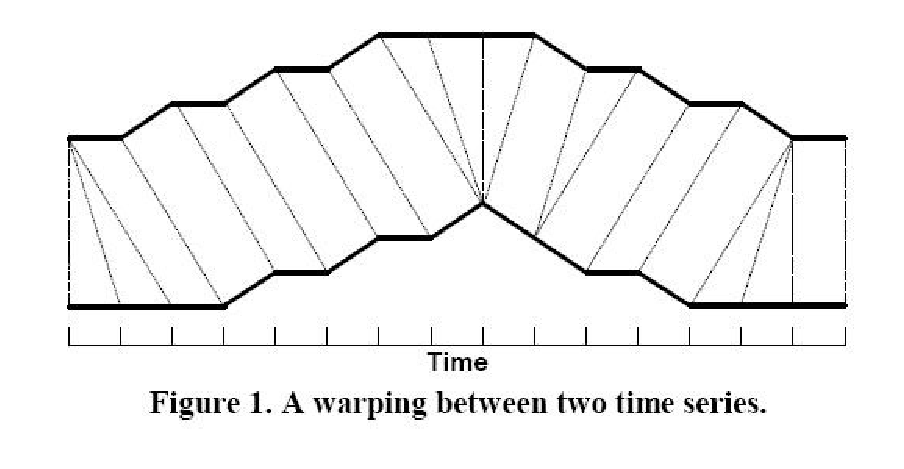
\includegraphics[height=4cm, width=5cm]{warping_two_series.eps}}
\caption{Alineamiento de tiempo distorsionado} \label{caja}
\end{figure}

En la Figura 2.1, cada l\'inea vertical conecta un punto en una serie temporal con su punto co\-rres\-pon\-dien\-te, similar en la otra serie temporal. Las l\'ineas realmente tienen valores similares en el eje vertical pero han sido separados, as\'i es que en las l\'ineas verticales entre ellos pueden ser miradas m\'as f\'acilmente.

Si ambas series temporales en la figura fueran id\'enticas, todas las l\'ineas ser\'ian l\'ineas directamente verticales porque todos los puntos ser\'ian similares entre ellos.

\subsection{Formulaci\'on del problema}
El problema del alineamiento de tiempo distorsionado es definido como sigue:

Dadas dos series de tiempo $X_{t}=(x_1,\ldots,x_{i},\ldots,x_m)$ e $Y_{t}=(y_1,\ldots,y_{j},\ldots,y_n)$ de largo $m$ y $n$ respectivamente. Se construye el camino distorsionado que llamaremos $W_{k}$, esta es una secuencia de pares de puntos ordenados, basado en los \'indices de las series $X_{t}$ e $Y_{t}$, donde:

$|r|=W_{k}=\{w_{1},\ldots,w_{K}\}$, $\max\{m,n\}\leq K\leq n\cdot m$. Adem\'as, $K=m \times n$ es la longitud m\'axima del camino distorsionado.
El camino distorsionado $W_{k}$ se define de la siguiente forma:

\begin{eqnarray}
w_{k}=(i,j), \mbox{    con $k=1,\ldots,K$}
\end{eqnarray}

donde $i$ es el \'indice de la Serie $X_t$ y $j$ es el \'indice de la serie $Y_t$.

El camino distorsionado debe empezar desde $w_{1}=(1,1)$ y el final de ambas en $w_K=(m,n)$. Esto asegura que cada \'indice de ambas serie temporales es usado en el camino distorsionado. Hay una restricci\'on en el camino distorsionado que obliga a $i$ y $j$ a ser monotonamente creciente.\\
Se define mas formalmente:

\[r=\left((x_{a_1},y_{b_1}),(x_{a_2},y_{b_2}),\ldots,(x_{a_m},y_{b_n})\right)=(w_{1},w_{2},\ldots,w_{K}),\]
con $a_{i}, i \in \{1,\ldots,n\}$,$b_{j}, j \in \{1,\ldots,n\}$ y satisfaciendo  para $i \in \{1,\ldots,m-1\}$ la siguiente condici\'on: $a_{1}=1$,$b_{n}=k$ $a_{i}=(a_{i}\mbox{   \'o   } a_{i+1})$ y $b_{j}=(b_{j}\mbox{  \'o     } b_{j+1})$.

Para detreminar DTW para dos secuencias de tiempo, construimos una matriz de $m\cdot n$ donde $(i^{th}, j^{th})$ son elementos de la matriz contiene la distancia $d(x_{a_i}, y_{b_i})$ entre los dos puntos $x_{a_i}$ e $y_{b_i}$, es decir,$d(x_{a_i}, y_{b_i})=|x_{a_i}-y_{b_i}|$. Cada elemento matricial $(i, j)$ corresponde a la alineaci\'on entre el punto de $x_{a_i}$ e $y_{b_i}$.

Este camino puede ser encontrado usando programaci\'on din\'amica para evaluar la siguiente recurrencia, que defina la distancia acumulativa $\gamma(i,j)$ como la distancia $d(i, j)$ encontrada en la celda actual y el m\'inimo de las distancias acumulativas de los elementos adyacentes,

\begin{eqnarray}
\gamma(i,j)&=&d(i,j)+min\{\gamma(i-1,j-1),\gamma(i-1,j),\gamma(i,j-1)\}.
\end{eqnarray}

\subsection{Hacia el Alineamiento de tiempo distorsionado}

El Alineamiento de tiempo distorsionado es un algoritmo para medir la similitud entre dos secuencias que pueden variar en el tiempo o en la velocidad. DTW se ha aplicado en video, audio y gr\'aficos, de hecho en cualquier dato que pueda ser convertido en una representaci\'on lineal se puede analizar con DTW.  Una conocida ha sido la aplicaci\'on autom\'atica de reconocimiento de voz, para hacer frente a diferentes velocidades haciendo uso de la palabra.

En general, DTW es un m\'etodo que permite a un ordenador encontrar una \'optima adecuaci\'on entre dos secuencias dadas (por ejemplo, series de tiempo), con ciertas restricciones.

Un ejemplo de las restricciones impuestas a la adecuaci\'on de las secuencias se encuentra en la monotocidad de la cartograf\'ia en la dimensi\'on temporal.  La continuidad es menos importante en DTW que en otros algoritmos de Coincidencia de patrones; DTW es un algoritmo especialmente adecuado para las secuencias de concordancia con la informaci\'on que falta.El proceso de optimizaci\'on se realiza utilizando programaci�n din\'amica, de ah\'i el nombre. Ejemplo de una de las muchas formas del algoritmo.
\begin{verbatim}
###############################################################################
#### RUTINA PARA DETERMINAR EL CAMINO DISTROSIONADO ###########################
  int DTWDistance (char s [1 .. n], char t [1 .. m], int d [1 .. n, 1 .. m]) (
      DTW declarar int [0 .. n, 0 .. m]
      declarar int i, j, el costo

      for i: = 1 to m
          DTW [0, i]: = infinito
      for i: = 1 hasta n
          DTW [i, 0]: = infinito
      DTW [0,0]: = 0

      for i: = 1 hasta n
          for j: = 1 to m
              coste: = d [s [i], t [j]]
              DTW [i, j]: = + costo m�nimo (DTW [i-1, j], / / inserci�n
                                         DTW [i, j-1], / / supresi�n
                                         DTW [i-1, j-1]) / / partido

      DTW retorno [n, m]
  )
##############################################################################
\end{verbatim}

Este algoritmo c\'alcula la distancia DTW para dos secuencias, donde los vectores pueden ser de distinto tama\~no. En la siguiente figura se puede apreciar que el algoritmo encuentra el camino mas corto entre dos series, que dependen de la similitud entre las mismas.

\begin{figure}[!htp]
\centering
\fbox{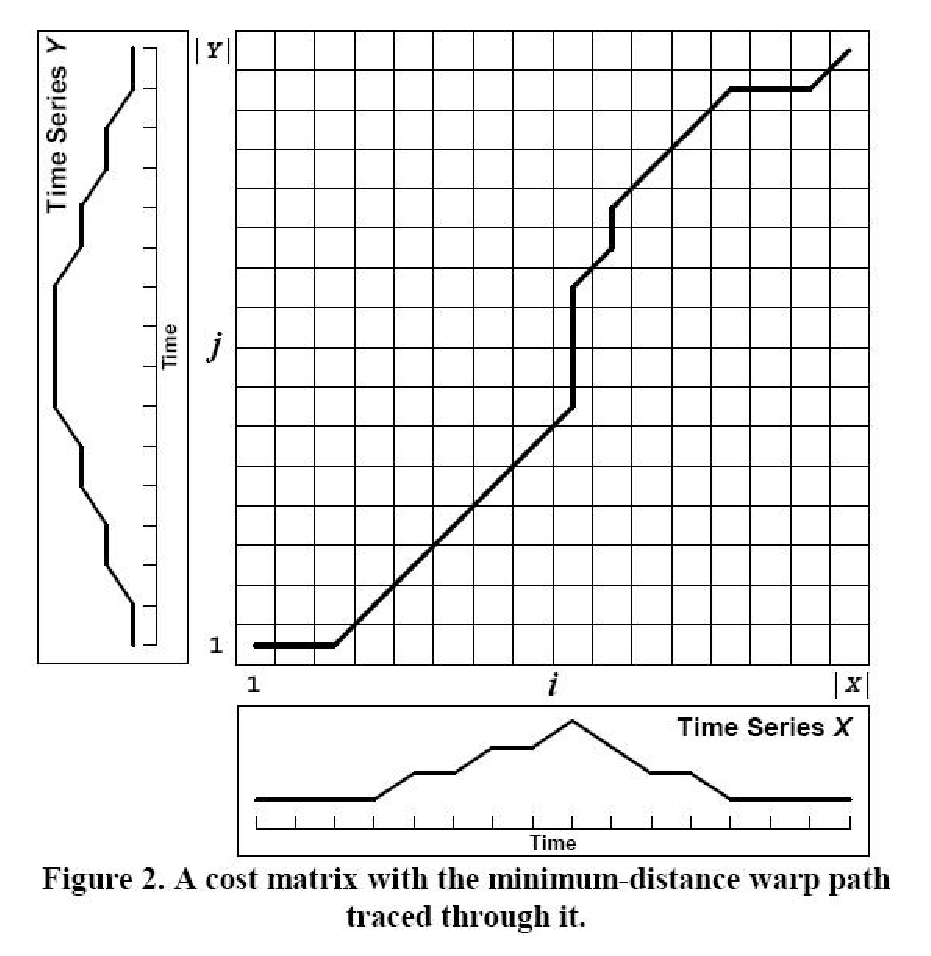
\includegraphics[height=4cm, width=5cm]{cost_minimun_distance.eps}}
\caption{Camino distorsionado} \label{caja}
\end{figure}

Ya mencionadas las caracter\'isticas se definir\'a mas formalmente la Distancia DTW.

\subsection{Definici\'on DTW}
Considere una nueva definici\'on de la rejilla propuesta en (2.3.3) como la suma de las distancias de todas las observaciones apareadas.
\begin{eqnarray}
|r|&=&\sum_{i=1}^{m}|x_{a_i}-y_{b_i}|.
\end{eqnarray}
Entonces la distancia $\delta_{DTW}$ se define de la siguiente manera:
\begin{eqnarray}
\delta_{DTW}(X_{t},Y_{t})&=&\min|r|=\min_{r\in M}\left(\sum_{i=1}^{m}|x_{a_i}-y_{b_i}|\right).
\end{eqnarray}

\subsection{Ejemplo}
La finalidad de este ejemplo es resumir esta secci\'on para dejar m\'as claro cuales son las bondades de DTW. Entonces, considere dos secuencias de tiempo. Sea $X_{t}=(1,0.34,0.65,2,3,3.4,1,1.2,0.88,5.9,7)$ e $Y_{t}=(2,5.5,5.67,3.45,7,3.3,2.43,1.34)$. Calcular $\delta_{DTW}(X_{t},Y_{t})$. Considere la siguiente rutina.

\begin{verbatim}
###############################################################################

library(dtw)
x<-c(1,0.34,0.65,2,3,3.4,1,1.2,0.88,5.9,7)
y<-c(2,5.5,5.67,3.45,7,3.3,2.43,1.34)
a<-dtw(x,y)
b<-a$distance
plot(a,xlab="indice de x",ylab="indice de y",main="Camino Distorcionado")
> length(x)
[1] 11
> length(y)
[1] 8
> b
[1] 26.45

#############################################################################
\end{verbatim}
En la salida de esta rutina se puede apreciar que la longitud del vector $X_{t}$ es de 11 elementos y la longitud del vector $Y_{t}$ es 8 elementos. Por otra parte la distancia es 26.45.\\
La opci\'on $\verb"plot(a)"$ en R muestra el siguiente gr\'afico.

\newpage
\begin{figure}[!htp]
\centering
\fbox{\includegraphics[height=5cm, width=7cm]{c_dtw.eps}}
\caption{Camino distorsionado de $\delta_{DTW}(X_{t},Y_{t})$.} \label{caja}
\end{figure}

Una de las caracter\'istica de DTW, es la representaci\'on gr\'afica de la similitud entre dos series temporales y en este caso se puede apreciar que las series no presentan un gran grado de similitud, ya que estos puntos no definen una linea recta.

Desde aqu\'i, se puede apreciar y entender m\'as f\'acilmente la definici\'on de camino distorsionado.

En esta secci\'on se han presentado las distancias $\delta_{E}$, $\delta_{M}$, $\delta_{F}$, y $\delta_{DTW}$ pero ellas ignoran la estructura temporal de los valores como proximidad, ya que, est\'an basada sobre las diferencias entre los valores $|x_{a_i}-y_{b_i}|$.

En la siguiente secci\'on se propondr\'a un \'Indice que considere la estructura de comovimiento y la cercan\'ia entre las series en el contexto de clasificaci\'on de series temporales.

\section{\'Indice de Disimilaridad Adaptativo para medidas de pro\-xi\-mi\-dad entre series de tiempo.}

Las medidas convencionales de proximidad en series temporales, est\'an basadas sobre la cercan\'ia de los valores observados de
las series de tiempo.

La idea de est\'a secci\'on es presentar un \'Indice  de Disimilaridad, que contenga la informaci\'on de la codipersi\'on o comovimiento y la cercan\'ia de las series temporales. En otras palabras se define la disimilaridad entre dos series de tiempo, considerando estas dos caracter\'isticas, uno el comportamiento respecto a su comovimiento y la otra sobre su cercan\'ia. Generalmente, se asume que esta medida entre las secuencias $X_t$ e $Y_t$ toman valores positivos.

Uno puede cuantificar el concepto de similaridad considerando el cl\'asico coeficiente de co\-rre\-la\-ci\'on de Pearson. Sin embargo, esta correlaci\'on gu\'ia una sobre estimaci\'on de la Codispersi\'on. De igual forma, el coeficiente de correlaci\'on de Spearman es tambi\'en usado como una medida de similaridad. No obstante, se ha visto que la correlaci\'on est\'a principalmente basada sobre los rangos y no sobre los  valores observados. Dejando de lado la informaci\'on respecto a su comovimiento.

\subsection{Correlaci\'on temporal para medidas de proximidad}
Ya se ha mencionado las desventajas de las medidas de distancias convencionales y los coeficientes de similaridad que no ayudan a establecer un \'indice que pueda conjugar estas dos ca\-rac\-te\-r\'is\-ti\-cas. Una estructura que considere la interdependencias entre dos serie puede deducirse considerando los siguientes elementos:

Sea $X_{t}=(x_1,\ldots,x_n)$ una colecci\'on de $n$ n\'umeros reales
independientes. La varianza cl\'asica de $X_{t}$ puede ser escrita en dos
vias equivalentes,
\begin{eqnarray}
Var(X_{t})=\frac{1}{n-1}{\sum_{i=1}^{n}(x_{i}-m)^2}=\frac{1}{n-1}{\sum_{i,i'}(x_i-m)^2},
\end{eqnarray}
donde $m$ es la media de los valores de $X_{t}$. Similarmente el coeficiente cl\'asico de correlaci\'on entre
$X_{t}=(x_1,\ldots,x_n)$ e $Y_{t}=(y_1,\ldots,y_n)$ puede ser escrito de dos formas:
\begin{eqnarray}
Corr_{X_{t},Y_{t}}=\frac{\sum_{i=i}^{n}(x_i-m_1)(y_i-m_2)}{\sqrt{Var({X_{t}})Var({Y_{t}})}}=\frac{\sum_{i,i'}(x_i-x_{i'})(y_i-y_{i'})}{\sqrt{\sum_{i,i'}(x_i-x_{i'})^{2}\sum_{i,i'}(y_i-y_{i'})^{2}}}.
\end{eqnarray}
En el caso general de medidas independientes varianza$/$covarianza y coeficiente de correlaci\'on son medidas basadas sobre la
contribuci\'on de todos los pares de medici\'on. A la inversa en el caso de las interdependencias se define una relaci\'on entre
vecino m\'as cercano.

La expresi\'on de la varianza puede ser descompuesta como sigue:
\begin{center}
\begin{eqnarray}
Var(X_{t})&=&\frac{1}{2n-1}{\sum_{i,i'}(x_i-x_{i'})^2}.
\end{eqnarray}
\end{center}

De igual forma,

\begin{eqnarray}
Var(S)&=&\frac{1}{2n-1}{\sum_{\mbox{$i$ es vecino de $i'$}}(x_i-x_{i'})^2}+\frac{1}{2n-1}{\sum_{\mbox{$i$ no es vecino de $i'$}}(x_i-x_{i'})^2}.
\end{eqnarray}

La idea principal para incluir la informaci\'on sobre la dependencia de las series, es una restricci\'on a la expresi\'on de la varianza$/$covarianza de los pares de valores dependientes (Vecinos).

\begin{eqnarray}
VarT(X_{t})=\frac{1}{2n-1}{\sum_{\mbox{$i$ no es vecino de $i'$}}(x_{i}-x_{i'})^2},
\end{eqnarray}

Para la similaridad, se considerara una relaci\'on temporal de
vecinos de orden $h$, medidas en el p\'eriodo ${[t_i,t_{i+h}]}$. Este coeficiente de
correlaci\'on temporal es definido como:

\begin{eqnarray}
\widehat{\rho}_{X_{t},Y_{t}}(h)=\frac{\sum_{i=i}^{n-1}(x_{i+h}-x_i)(y_{i+h}-y_{i})}{\sqrt{\sum_{i=1}^{n-1}(x_{i+h}-x_i)^{2}\sum_{i=i}^{n-1}(y_{i+h}-y_{i})^{2}}}.
\end{eqnarray}

donde $\widehat{\rho}_{X_{t},Y_{t}}(h)$ pertenece al intervalo $[-1,1]$. La interpretaci\'on de los valores se discuti\'o  en la secci\'on de ejemplos en el cap\'itulo I.

\subsection{\'Indice de Disimilaridad Adaptativo entre series de tiempo}

El prop\'osito de este cap\'itulo es apuntar a un nuevo \'Indice con aspiraci\'on a cubrir ambas medidas convencionales de similaridad y cercan\'ia
para la proximidad de valores y la correlaci\'on temporal entre dos series temporales para medir el comportamiento conjunto.


El resultado de la medida de disimilaridad debe tambi\'en permitir ajustar el peso de la contribuci\'on entre ambos cuantiles (Comovimiento y Cercan\'ia). Para ajustar el peso de la contribuci\'on de los cuantiles es necesario tener una funci\'on  $f(x)$ que module la distancia incrementando o dis\-mi\-nu\-yen\-do las medidas convencionales antes definidas.


Conforme con las especificaciones anteriores, se propone un \'Indice de Disimilaridad $D(X_{t},Y_{t})$ basado sobre una funci\'on de afinaci\'on autom\'atica que module el comportamiento de las medidas convencionales.


Ahora bien, en el contexto de an\'alisis de grupos (Cluster) Chouakria y  Na\-ga\-bhu\-shan (2007) propusieron un \'Indice de Disimilaridad Adaptativo para medidas de proximidad en series temporales, como una nueva medida de distancia, la cual definieron de la siguiente forma,

\begin{eqnarray}
D({X_{t}},{Y_{t}})&=&f(\widehat{\rho}_{X_{t},Y_{t}}(h))\delta_{C}({X_{t}},{Y_{t}}),
\end{eqnarray}

donde $f(x)$ es una funci\'on de afinaci\'on exponencial adaptativa, es dado por

\begin{eqnarray}
 f(x)&=&\frac{2}{1+exp(kx)},\mbox{  $k \geq 0$}.
\end{eqnarray}

y $\delta_{C}({X_{t}},{Y_{t}})$ es cualquier distancia convencional entre ${X_{t}}$ e ${Y_{t}}$. Note que la funci\'on $f(x)$ depende del estimador muestral del Coeficiente de Codispersi\'on. En la Figura 2.4, se puede apreciar la funci\'on de afinamiento adaptativo para distintos valores de $k$.

\begin{figure}[!htp]
\centering
\fbox{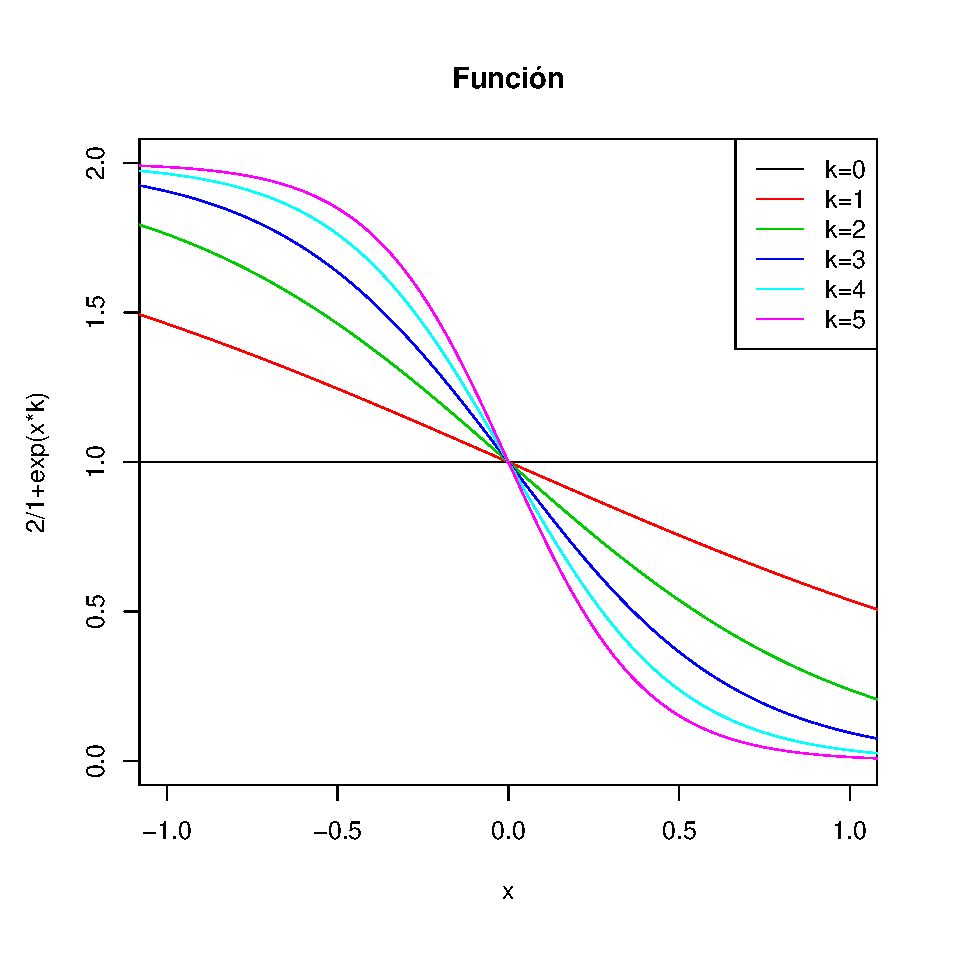
\includegraphics[height=5cm, width=6cm]{fat.eps}}
\caption{Funci\'on exponencial adaptativo} \label{caja}
\end{figure}
\newpage
La funci\'on de $k$ es modular con m\'as o menos fuerza la contribuci\'on de los cuantiles sobre las medidas convencionales. Esto se puede apreciar en la tabla.

\begin{center}
\begin{small}
\begin{tabular}{|l|l|l|l}
\cline{1-3}
\multicolumn{3}{|c|}{Contribuci\'on en \% de $k$ con respecto a } &  \\
\cline{1-3}
\multicolumn{1}{|c|}{$k$} & \multicolumn{1}{c|}{$f(x)$ } & \multicolumn{1}{c|}{$D(X_{t},Y_{t})$} &  \\
\cline{1-3}
\multicolumn{1}{|c|}{0} & \multicolumn{1}{c|}{0} & \multicolumn{1}{c|}{100} &  \\
\multicolumn{1}{|c|}{1} & \multicolumn{1}{c|}{46.2} & \multicolumn{1}{c|}{53.7} &  \\
\multicolumn{1}{|c|}{2} & \multicolumn{1}{c|}{76.2} & \multicolumn{1}{c|}{23.8} &  \\
\multicolumn{1}{|c|}{3} & \multicolumn{1}{c|}{90.5} & \multicolumn{1}{c|}{9.4} &  \\
\multicolumn{1}{|c|}{$\geq$ 5} & \multicolumn{1}{c|}{$\approx$100} & \multicolumn{1}{c|}{$\approx$0} &  \\
\cline{1-3}
\end{tabular}
\end{small}
\end{center}

Por ejemplo, cuando $k=0$ y $f(0)=1$, el \'Indice de Disimilaridad est\'a representado s\'olo por la distancia convencional y estamos en presencia de una medida de semejanza cl\'asica, para los algoritmos de clasificaci\'on en Cluster.

Con este nuevo \'Indice de Disimilaridad se espera captar mejor la correlaci\'on temporal que las medidas
convencionales de distancias para clasificaci\'on de series temporales.

Este \'Indice de disimilaridad es una medida alternativa
para clasificar series temporales a los m\'etodos cl\'asicos que
se conocen. Un m\'etodo de clasificaci\'on que depende de este \'indice de disimilaridad sera presentada en el Cap\'itulo III.



